\usetikzlibrary{calc}
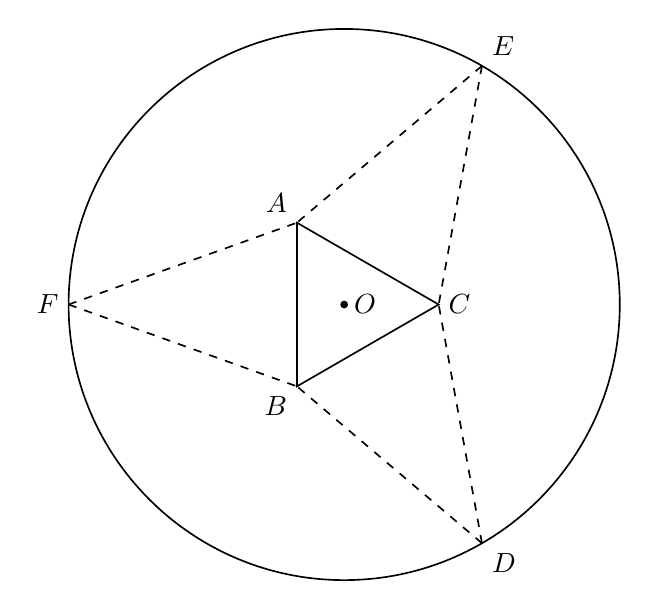
\begin{tikzpicture}[x=1cm,y=1cm,line width=.6pt,font=\normalsize]
\coordinate (O) at (0,0);
\coordinate (A) at (-0.6,1.0392305);
\coordinate (B) at (-0.6,-1.0392305);
\coordinate (C) at (1.2,0);
\coordinate (D) at (1.75,-3.0310889);
\coordinate (E) at (1.75,3.0310889);
\coordinate (F) at (-3.5,0);
\draw (O) circle[radius=3.5cm];
\draw (A)--(B)--(C)--cycle;
\draw[dashed] (D)--(B);
\draw[dashed] (D)--(C);
\draw[dashed] (E)--(C);
\draw[dashed] (E)--(A);
\draw[dashed] (F)--(A);
\draw[dashed] (F)--(B);
\fill (O) circle[radius=1.4pt];
\node[above left] at (A) {$A$};
\node[below left] at (B) {$B$};
\node[right] at (C) {$C$};
\node[below right] at (D) {$D$};
\node[above right] at (E) {$E$};
\node[left] at (F) {$F$};
\node[right] at (O) {$O$};
\end{tikzpicture}
